\documentclass[sigconf,nonacm]{acmart}

\usepackage{amsmath}
\usepackage{booktabs}
\usepackage{graphicx}
\usepackage{placeins}
\usepackage{tabularx}

\graphicspath{{figures/}}
\settopmatter{printacmref=false,printccs=false}

\newcolumntype{Y}{>{\raggedright\arraybackslash}X}

\newcommand{\dataset}{\mathcal{D}}
\newcommand{\retained}{\mathcal{D}'}
\newcommand{\queries}{\mathcal{Q}}
\newcommand{\budget}{B}
\newcommand{\cosim}{\operatorname{cos}}
\newcommand{\argmax}{\operatorname*{arg\,max}}

\title[Query-Aware Photo Selection]{Query-Aware Photo Selection for Data Reduction}
\author{Luca Foresti}
\authornote{Matricola: 565562. Documentation refreshed June 28, 2026.}
\affiliation{%
  \institution{Roma Tre University}
  \city{Rome}
  \country{Italy}
}
\date{June 28, 2026}
\renewcommand{\shortauthors}{Foresti}

\begin{document}
\begin{abstract}
This project studies a practical data-reduction task from the course assignment~\cite{velegrakis2026practical}: given photo embeddings and a historical query log, choose a budgeted subset of photos to retain while preserving query usefulness. I implement the three required baselines, exhaustive cosine search (A), IndepDF query-membership scoring (B), and exact Shapley ranking (C), and propose Method D, a query-weighted greedy facility-location method. The private dataset has 41,620 photos, 2,048 embedding dimensions, and 443 query rows. Exact methods are useful only on tiny samples, Method B is the fastest scalable baseline, and Method D gives the strongest scalable cosine-proxy utility while remaining feasible on the full dataset.
\end{abstract}

\maketitle

\section{Problem and Data Contract}

The assignment gives a photo matrix \texttt{photos.csv} and a query log \texttt{queries.csv}. Each photo $d \in \dataset$ is an embedding vector, and each query row lists photo identifiers returned by one historical search. The objective is to retain at most $\budget$ photos:
\begin{equation}
  \retained^{*} =
  \argmax_{\retained \subseteq \dataset,\ |\retained| \leq \budget}
  \mathbb{E}_{q \sim \queries}\left[S(q(\dataset), \retained)\right].
  \label{eq:main-objective}
\end{equation}

The original query operators are unavailable, so the implementation uses historical results as empirical evidence of what should remain useful. I report two metrics. The primary metric is a cosine replacement proxy:
\begin{equation}
  S(q(\dataset), \retained)
  =
  \frac{1}{|q(\dataset)|}
  \sum_{d \in q(\dataset)}
  \max_{s \in \retained} \cosim(d, s).
  \label{eq:cosine-proxy}
\end{equation}
The secondary metric is membership precision, the fraction of historical query results directly retained.

The loader treats the assignment photo ID as the line number in \texttt{photos.csv}, so canonical raw-data runs use one-based query IDs and then normalize to zero-based internal IDs. CSV validation rejects malformed photo rows, nonnumeric values, missing values, empty query rows, duplicate query IDs, and out-of-range IDs. In the validated private dataset, the query log references 10,937 distinct target photos after normalization.

\section{Methods}

All methods share the same selection interface, budget validation, normalized photo matrix, query rows, deterministic lower-ID tie-breaking, timing, memory measurement, and diagnostics. Exact methods return a documented \texttt{skipped} result when a configured guardrail is exceeded.

\begin{table*}[!htbp]
  \centering
  \caption{Implemented methods and their role in the comparison.}
  \label{tab:methods}
  \small
  \begin{tabularx}{\textwidth}{@{}lYYY@{}}
    \toprule
    Method & Signal & Optimization & Role \\
    \midrule
    A & Cosine proxy & Exhaustive subset search & Exact tiny baseline \\
    B & Query membership & IndepDF score ranking & Scalable query baseline \\
    C & Cosine proxy & Exact Shapley ranking & Principled tiny baseline \\
    D & Query weights + cosine & Greedy facility location & Proposed scalable method \\
    \bottomrule
  \end{tabularx}
\end{table*}

\subsection{Method A: exhaustive cosine search}
Method A enumerates all size-$\budget$ subsets and returns the subset with maximum cosine-proxy utility. It is the cleanest correctness reference on tiny samples, but its $\binom{m}{\budget}$ search space makes it infeasible on the full collection.

\subsection{Method B: IndepDF query scoring}
Method B scores each photo by its average normalized membership mass:
\begin{equation}
  \operatorname{score}(d)
  =
  \mathbb{E}_{q \sim \queries}
  \left[
    \frac{I_q(d)}{|q(\dataset)|}
  \right],
  \label{eq:indepdf}
\end{equation}
where $I_q(d)=1$ if $d$ appears in query result $q(\dataset)$ and $0$ otherwise. It is extremely fast and memory-light, but it does not use embedding similarity or diversity.

\subsection{Method C: exact Shapley ranking}
Method C computes the exact Shapley value of each photo under the cosine-proxy utility and selects the top $\budget$ photos~\cite{shapley1953value}:
\begin{equation}
  \phi_d =
  \sum_{T \subseteq \dataset \setminus \{d\}}
  \frac{|T|!(m-|T|-1)!}{m!}
  \left(f(T \cup \{d\}) - f(T)\right).
  \label{eq:shapley}
\end{equation}
This gives a principled individual contribution score, but exact coalition enumeration is exponential, so the implementation only runs it on small samples.

\subsection{Method D: query-aware facility location}
Method D is the proposed method. It follows the workload-aware data-forgetting perspective of retaining data that preserves downstream utility~\cite{rico2026stochastic}. It assigns each photo a query-derived weight $w_d$ using the same normalized query mass as Method B, then greedily maximizes weighted clipped cosine coverage:
\begin{equation}
  F(S) =
  \sum_{d \in \dataset}
  w_d \max_{s \in S} \max(0, \cosim(d, s)).
  \label{eq:facility}
\end{equation}
At each step it maintains the best current similarity for every positively weighted target and selects the candidate with the largest marginal gain. Negative cosines are clipped to zero so that a retained photo can only provide positive replacement evidence. Candidate evaluation is chunked by a configurable memory limit, so Method D can run on the full dataset without building a dense all-pairs similarity matrix.

\begin{table*}[!htbp]
  \centering
  \caption{Cost drivers. Here $m$ is candidate photos, $r$ total query memberships, $t$ positively weighted targets, $k$ budget, and $c$ the Method D candidate chunk size.}
  \label{tab:complexity}
  \small
  \begin{tabularx}{\textwidth}{@{}lYY@{}}
    \toprule
    Method & Main time cost & Main memory cost \\
    \midrule
    A & $\mathcal{O}\!\left(\binom{m}{k}\cdot\mathrm{eval}\right)$ & selected subset and evaluation buffers \\
    B & $\mathcal{O}(r + m\log m)$ & score vector of length $m$ \\
    C & $\mathcal{O}(2^m\cdot m\cdot\mathrm{eval})$ & coalition values and Shapley scores \\
    D & $\mathcal{O}(k\cdot m\cdot t)$ similarities, chunked & $\mathcal{O}(t\cdot c)$ similarity chunk \\
    \bottomrule
  \end{tabularx}
\end{table*}

\section{Final Answer}

The smallest assignment budget is $\budget=3$. The full-data Method D run is the recommended retained set because it uses both historical query importance and embedding replacement quality.

\begin{table*}[!htbp]
  \centering
  \caption{Recommended full-data output for $\budget=3$. Normalized IDs are zero-based internal IDs; assignment line IDs are one-based photo IDs.}
  \label{tab:final-answer}
  \small
  \begin{tabularx}{\textwidth}{@{}lYrrr@{}}
    \toprule
    Method & Selected photos & Cosine proxy & Runtime (s) & Peak MB \\
    \midrule
    D & normalized: 5974, 39809, 24228; line IDs: 5975, 39810, 24229 & 0.369236 & 31.172 & 427.795 \\
    \bottomrule
  \end{tabularx}
\end{table*}

This set should be read as the output of the implemented objective, not as a universal statement that these are intrinsically the best personal photos. If a deployment needed an immediate low-resource answer, Method B is the fallback; for offline selection under storage pressure, Method D is the stronger choice.

\section{Experiments}

Experiments are driven by YAML configs and saved as tidy CSV rows plus diagnostics JSON. Figures are regenerated from saved result files rather than manually edited spreadsheets. The canonical evidence uses the private raw dataset with one-based query IDs.

\begin{table*}[!htbp]
  \centering
  \caption{Canonical evidence batches used for the report.}
  \label{tab:batches}
  \small
  \begin{tabularx}{\textwidth}{@{}lYl@{}}
    \toprule
    Batch & Purpose & Methods \\
    \midrule
    \texttt{synthetic\_canonical} & deterministic clustered smoke tests & A, B, C, D \\
    \texttt{small\_exact\_comparison\_canonical} & compare all methods where exact A/C are feasible & A, B, C, D \\
    \texttt{scalability\_canonical} & scale B and D from 1,000 photos to the full dataset & B, D \\
    \texttt{budget\_sensitivity\_canonical} & test budgets 1, 3, 5, 10, and 25 on 10,000 photos & B, D \\
    \texttt{d\_ablations\_canonical} & isolate query weighting and embedding coverage & D variants \\
    \texttt{query\_holdout\_canonical} & train on 75\% of projected queries and evaluate on 25\% & B, D \\
    \texttt{exact\_infeasibility\_canonical} & document full-data skips for exact A and C & A, C \\
    \bottomrule
  \end{tabularx}
\end{table*}

\subsection{Exact methods}
On the full dataset, Method A would need to evaluate 12,014,997,\allowbreak{}156,340 subsets for $\budget=3$, and 125,007,034,\allowbreak{}163,850,\allowbreak{}445 subsets for $\budget=4$. Method C is even less feasible because exact Shapley values require coalition enumeration. The code therefore skips full-data A and C with explicit diagnostics rather than silently omitting them.

\subsection{Small exact comparison}
On query-active samples small enough for exact search, Method D nearly matches Method A under the cosine proxy. For $\budget=3$, average cosine utility is 0.612920 for A and 0.612436 for D. For $\budget=4$, it is 0.696715 for A and 0.696319 for D. This is evidence that the greedy coverage objective recovers the exact coverage structure on feasible instances.

\subsection{Scalability and quality}
Method B is consistently fastest and lightest. On the full dataset at $\budget=3$, B runs in 0.022 seconds with 1.278 MB peak measured memory, but its cosine-proxy utility is 0.283321. Method D runs in 31.172 seconds with 427.795 MB peak measured memory and reaches 0.369236 cosine-proxy utility. Averaged over the scalability batch, B reaches 0.293034 while D reaches 0.366595.

\begin{figure*}[!htbp]
  \centering
  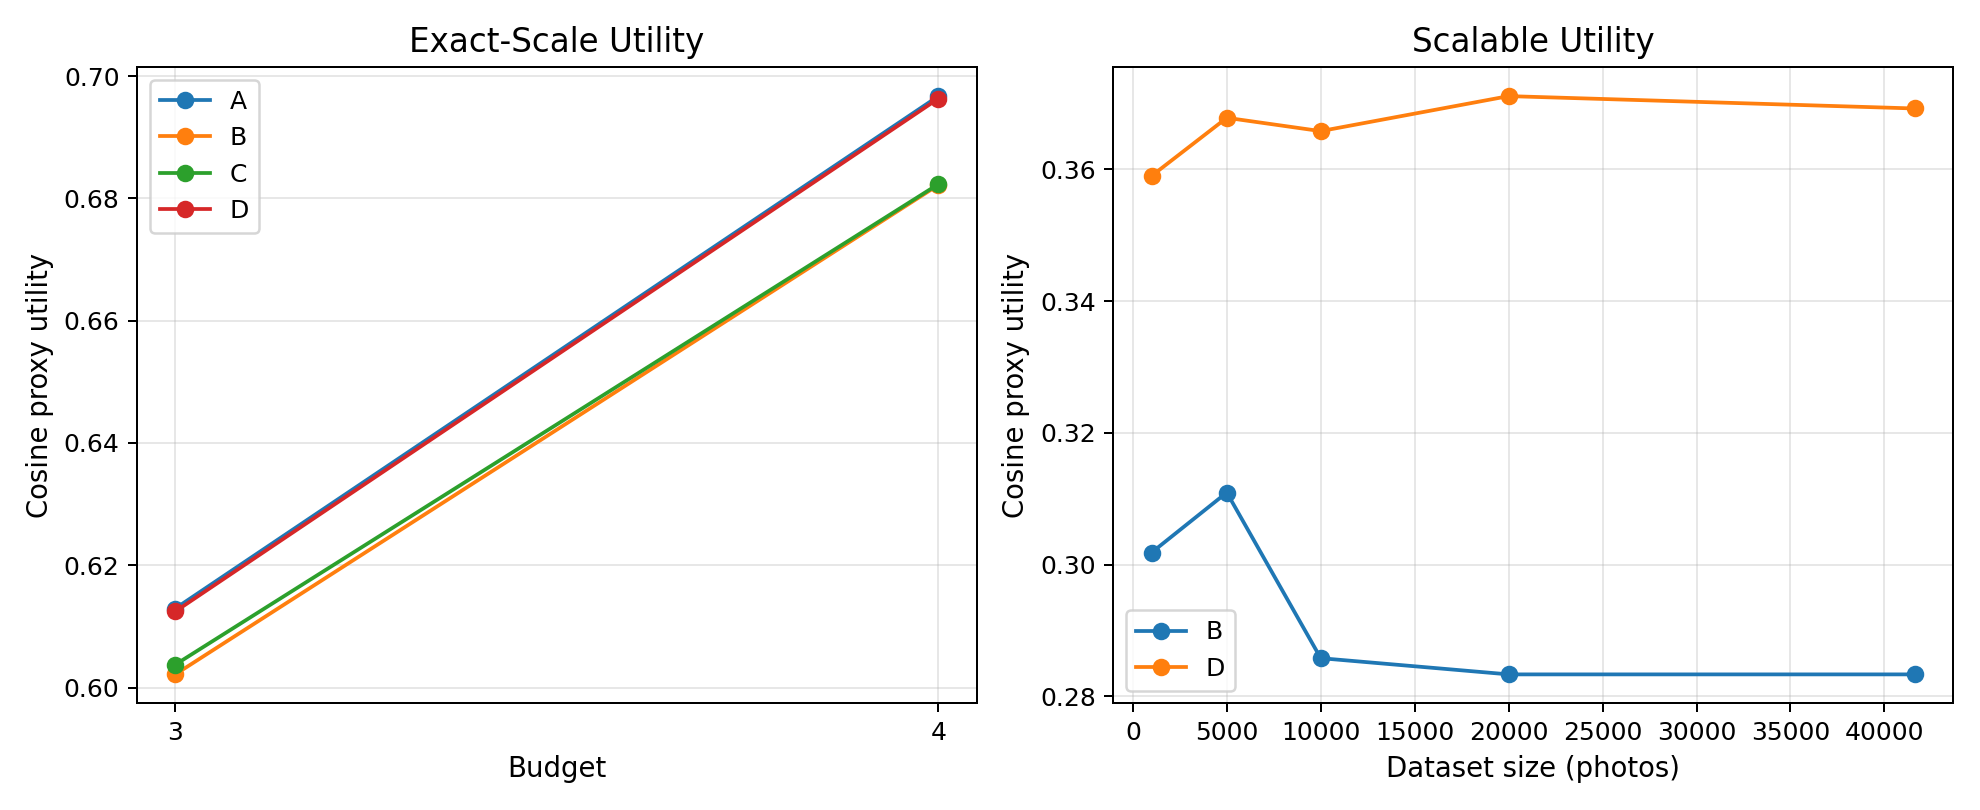
\includegraphics[width=\textwidth]{utility.png}
  \caption{Cosine-proxy utility. Method D tracks exact search on tiny samples and improves over Method B on scalable runs.}
  \Description{Line and bar plots comparing cosine-proxy utility across methods and dataset sizes, showing Method D close to exact search on tiny samples and above Method B on scalable runs.}
  \label{fig:utility}
\end{figure*}

\begin{table}[!htbp]
  \centering
  \caption{Scalability rows for the two full-data-capable methods at $\budget=3$.}
  \label{tab:scalability-rows}
  \small
  \begin{tabular}{@{}lrrr@{}}
    \toprule
    Method & Photos & Cosine proxy & Runtime (s) \\
    \midrule
    B & 1,000 & 0.302 & 0.012 \\
    B & 5,000 & 0.311 & 0.015 \\
    B & 10,000 & 0.286 & 0.017 \\
    B & 20,000 & 0.283 & 0.021 \\
    B & 41,620 & 0.283 & 0.022 \\
    D & 1,000 & 0.359 & 0.229 \\
    D & 5,000 & 0.368 & 2.205 \\
    D & 10,000 & 0.366 & 7.240 \\
    D & 20,000 & 0.371 & 15.178 \\
    D & 41,620 & 0.369 & 31.172 \\
    \bottomrule
  \end{tabular}
\end{table}

\begin{figure*}[!htbp]
  \centering
  
\includegraphics[width=\textwidth]{scalability.png}
  \caption{Runtime and memory scaling for Methods B and D. Method D is more expensive but remains feasible on the full dataset through chunked similarity coverage.}
  \Description{Runtime and memory scaling plots for Methods B and D across increasing photo counts, with Method D using more resources but remaining feasible on the full dataset.}
  \label{fig:scalability}
\end{figure*}

\begin{figure*}[!htbp]
  \centering
  \begin{minipage}[t]{0.49\textwidth}
    \centering
    
\includegraphics[width=\linewidth]{runtime.png}
  \end{minipage}\hfill
  \begin{minipage}[t]{0.49\textwidth}
    \centering
    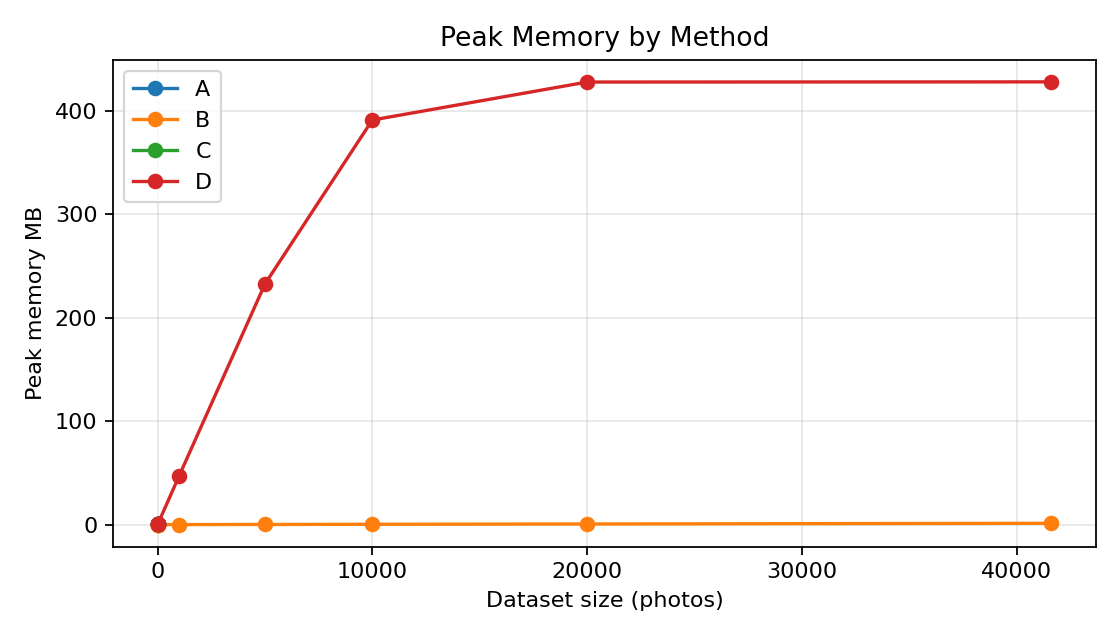
\includegraphics[width=\linewidth]{memory.png}
  \end{minipage}
  \caption{Runtime and peak measured memory by method and dataset size. Exact methods appear only on tiny samples; B is effectively instantaneous, while D pays more runtime and memory for embedding coverage.}
  \Description{Two plots side by side: runtime by method and dataset size, and peak memory by method and dataset size. Method B stays low while Method D increases with scale.}
  \label{fig:runtime-memory}
\end{figure*}

\subsection{Budget sensitivity and holdout}
On the 10,000-photo budget-sensitivity batch, D improves from 0.293731 at $\budget=1$ to 0.471688 at $\budget=25$, while B improves from 0.218811 to 0.431440. In the query-holdout batch, averaged over budgets and seeds, held-out cosine-proxy utility is 0.399460 for D and 0.295733 for B. The holdout split is random because the query log has no timestamps, but it reduces the risk that D only fits the exact query rows used for scoring.

The Method D ablation batch supports the combined objective. Full D averages 0.422695 cosine-proxy utility. Coverage only reaches 0.421382, while frequency only reaches 0.352703. Frequency weighting retains more direct query membership but loses embedding coverage when used without the coverage objective.

\begin{figure*}[!htbp]
  \centering
  \begin{minipage}[t]{0.49\textwidth}
    \centering
    
\includegraphics[width=\linewidth]{budget_sensitivity.png}
  \end{minipage}\hfill
  \begin{minipage}[t]{0.49\textwidth}
    \centering
    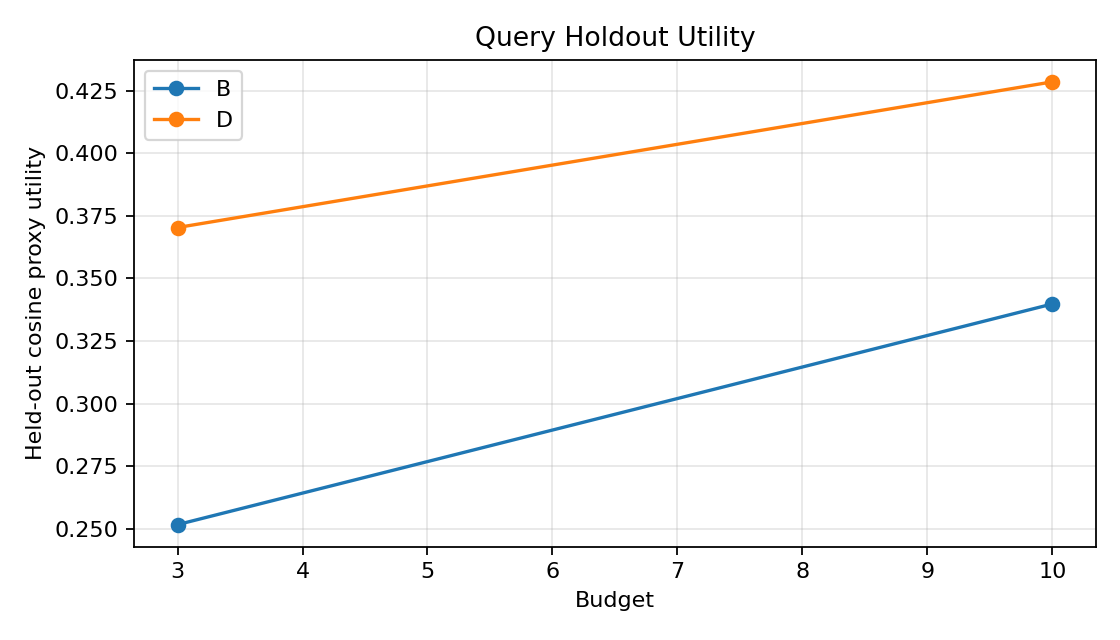
\includegraphics[width=\linewidth]{holdout_utility.png}
  \end{minipage}
  \caption{Budget sensitivity and held-out query utility. D gains more embedding-level utility as the retention budget grows and remains stronger than B on held-out queries.}
  \Description{Two plots side by side: budget sensitivity for Methods B and D, and held-out query utility for Methods B and D. Method D is higher in both plots.}
  \label{fig:budget-holdout}
\end{figure*}

\FloatBarrier

\section{Discussion}

The methods expose a clear cost-quality trade-off. Method A is the exact cosine-proxy optimum on tiny samples but cannot scale. Method B is a strong engineering baseline because it is simple, deterministic, and essentially instantaneous, but it only preserves direct historical memberships. Method C is conceptually useful as a game-theoretic individual contribution baseline, but exact computation is not practical at assignment scale. Method D is the best compromise: it uses query history to decide which regions matter and cosine coverage to avoid wasting budget on redundant photos.

\begin{table*}[!htbp]
  \centering
  \caption{Overall comparison.}
  \label{tab:overall}
  \small
  \begin{tabularx}{\textwidth}{@{}lYYYY@{}}
    \toprule
    Method & Strength & Weakness & Scale & Recommendation \\
    \midrule
    A & exact under chosen proxy & combinatorial search & tiny only & correctness reference \\
    B & fastest, lowest memory & no embedding coverage & full data & emergency fallback \\
    C & principled contribution score & exponential exact version & tiny only & diagnostic baseline \\
    D & best scalable cosine utility & slower and heavier than B & full data & final offline method \\
    \bottomrule
  \end{tabularx}
\end{table*}

The main limitation is that cosine-proxy utility is not the true user utility. It is a reproducible proxy made necessary by the absence of original query operators. The second limitation is workload drift: future searches may differ from historical searches. A production mobile system should also support user constraints such as favorites, albums, and recent photos. Within the assignment setting, however, Method D is the most appropriate final strategy because it is workload-aware, embedding-aware, deterministic, and feasible on the full private dataset.

\FloatBarrier

\section{Reproducibility}

The repository is a Python 3.12 project managed with \texttt{uv}. Raw data is intentionally ignored by git; a clean clone requires placing \texttt{photos.csv} and \texttt{queries.csv} under \texttt{data/raw/}. Core verification commands are:
\begin{verbatim}
uv sync
uv run python scripts/validate_data.py --id-base one
uv run pytest
uv run ruff check .
uv run python scripts/generate_figures.py \
  --results experiments/results \
  --output experiments/figures
\end{verbatim}
The automated tests cover CSV validation, ID normalization, invalid data, cosine similarity, utility metrics, method determinism, exact-method skips, Method D chunking, experiment expansion, holdout evaluation, diagnostics, and figure generation.

\section{Conclusion}

This project implements all required methods and evaluates them under a shared, reproducible pipeline. The final recommendation is Method D with $\budget=3$, retaining assignment line IDs 5975, 39810, and 24229. Method D is not exact, and it is more expensive than IndepDF, but it best matches the assignment goal: reduce the photo collection while preserving expected search usefulness from both historical query evidence and embedding-level replacement quality.

\bibliographystyle{ACM-Reference-Format}
\bibliography{references}

\end{document}
